\documentclass[11pt,xcolor=dvipsnames,professionalfonts]{beamer}

% Pakete
\usepackage[utf8]{inputenc}
\usepackage[english]{babel}

% AMS Pakete
\usepackage{amsmath}
\usepackage{amsfonts}
\usepackage{amssymb}

% Einheiten
\usepackage{siunitx}
\sisetup{
	separate-uncertainty
}

% Grafiken
\usepackage{graphicx}
\usepackage{tabularx}
\setbeamerfont{caption}{size=\footnotesize}
\setbeamertemplate{caption}{\raggedright\insertcaption\par}

% Theme
\usetheme{Boadilla}
\usecolortheme{rose}
\useoutertheme{infolines}
\useinnertheme{rectangles}
\setbeamertemplate{itemize subitem}[triangle]

\usefonttheme[onlymath]{serif}

% [num] Zitationen
\setbeamertemplate{bibliography item}[text]

% Navigationsleiste ausschalten
\beamertemplatenavigationsymbolsempty

\author[Christopher Deutsch]
{Christopher Deutsch}

\title
{Interactions of photons with matter}

\subtitle
{}
%\logo{}

\institute[]
{Rheinische Friedrich-Wilhelms-Universität Bonn \\
Seminar on Detectors in Nuclear and Particle Physics -- SS16}

\date{2.\ May 2016}

%\setbeamercovered{transparent}
%\setbeamertemplate{navigation symbols}{}

\newcommand{\beginbackup}{
	\newcounter{framenumbervorappendix}
	\setcounter{framenumbervorappendix}{\value{framenumber}}
}
\newcommand{\backupend}{
	\addtocounter{framenumbervorappendix}{-\value{framenumber}}
	\addtocounter{framenumber}{\value{framenumbervorappendix}} 
}

\begin{document}
\maketitle

\begin{frame}{Interactions of photons with matter}
	\tableofcontents
\end{frame}

\begin{frame}{Keywords}
	\begin{itemize}
		\item Photoelectric effect
		
		\item Compton effect
		
		\item Pair production
		
		\item Electromagnetic showers
		
		\item Detector concepts		
	\end{itemize}
\end{frame}

\section{Introduction}

\subsection{Charged particle interaction}

\begin{frame}{Introduction -- Interactions of charged particles with matter}
	last week: interactions of charged particles with matter
	\begin{itemize}
		\item energy loss due to inelastic collisions with atomic electrons
	\end{itemize}
	\vfill
	\begin{center}
		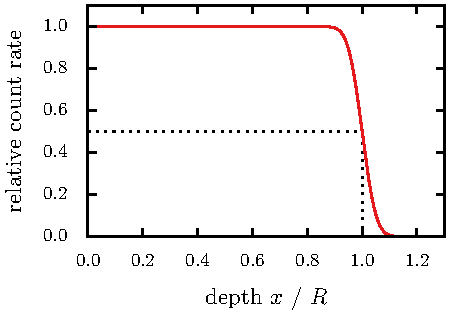
\includegraphics{./figures/range.pdf}
	\end{center}
\end{frame}


\subsection{Photon interaction}

\begin{frame}{Introduction -- Interactions of photons with matter}
	Today: photons (whats different?)
	\begin{itemize}
		\item uncharged
		
		\item relevant processes: photoelectric effect, compton scattering, pair production (etc.?) (why?)
		
		\item more penetrating than charged particles 
		\begin{itemize}
			\item lower cross section than inelastic electron collision
		\end{itemize}
		
		\item single photons in a beam don not lose energy, but the intensity of the beam drops
		\begin{itemize}
			\item interaction removes photon from beam entirely
			
			\item Lambert-Beer law ("derive"):
			\begin{align*}
				I(x) = I_0 \, e^{- \mu x}
			\end{align*}
			
			\item compare with stopping power for charged particles
		\end{itemize}
	\end{itemize}
\end{frame}

\begin{frame}{Lambert-Beer law}
	\begin{columns}
		\column[t]{0.6\textwidth}
			\begin{itemize}
				\item charge
			\end{itemize}
		
		\column[t]{0.4\textwidth}		
			\begin{center}
				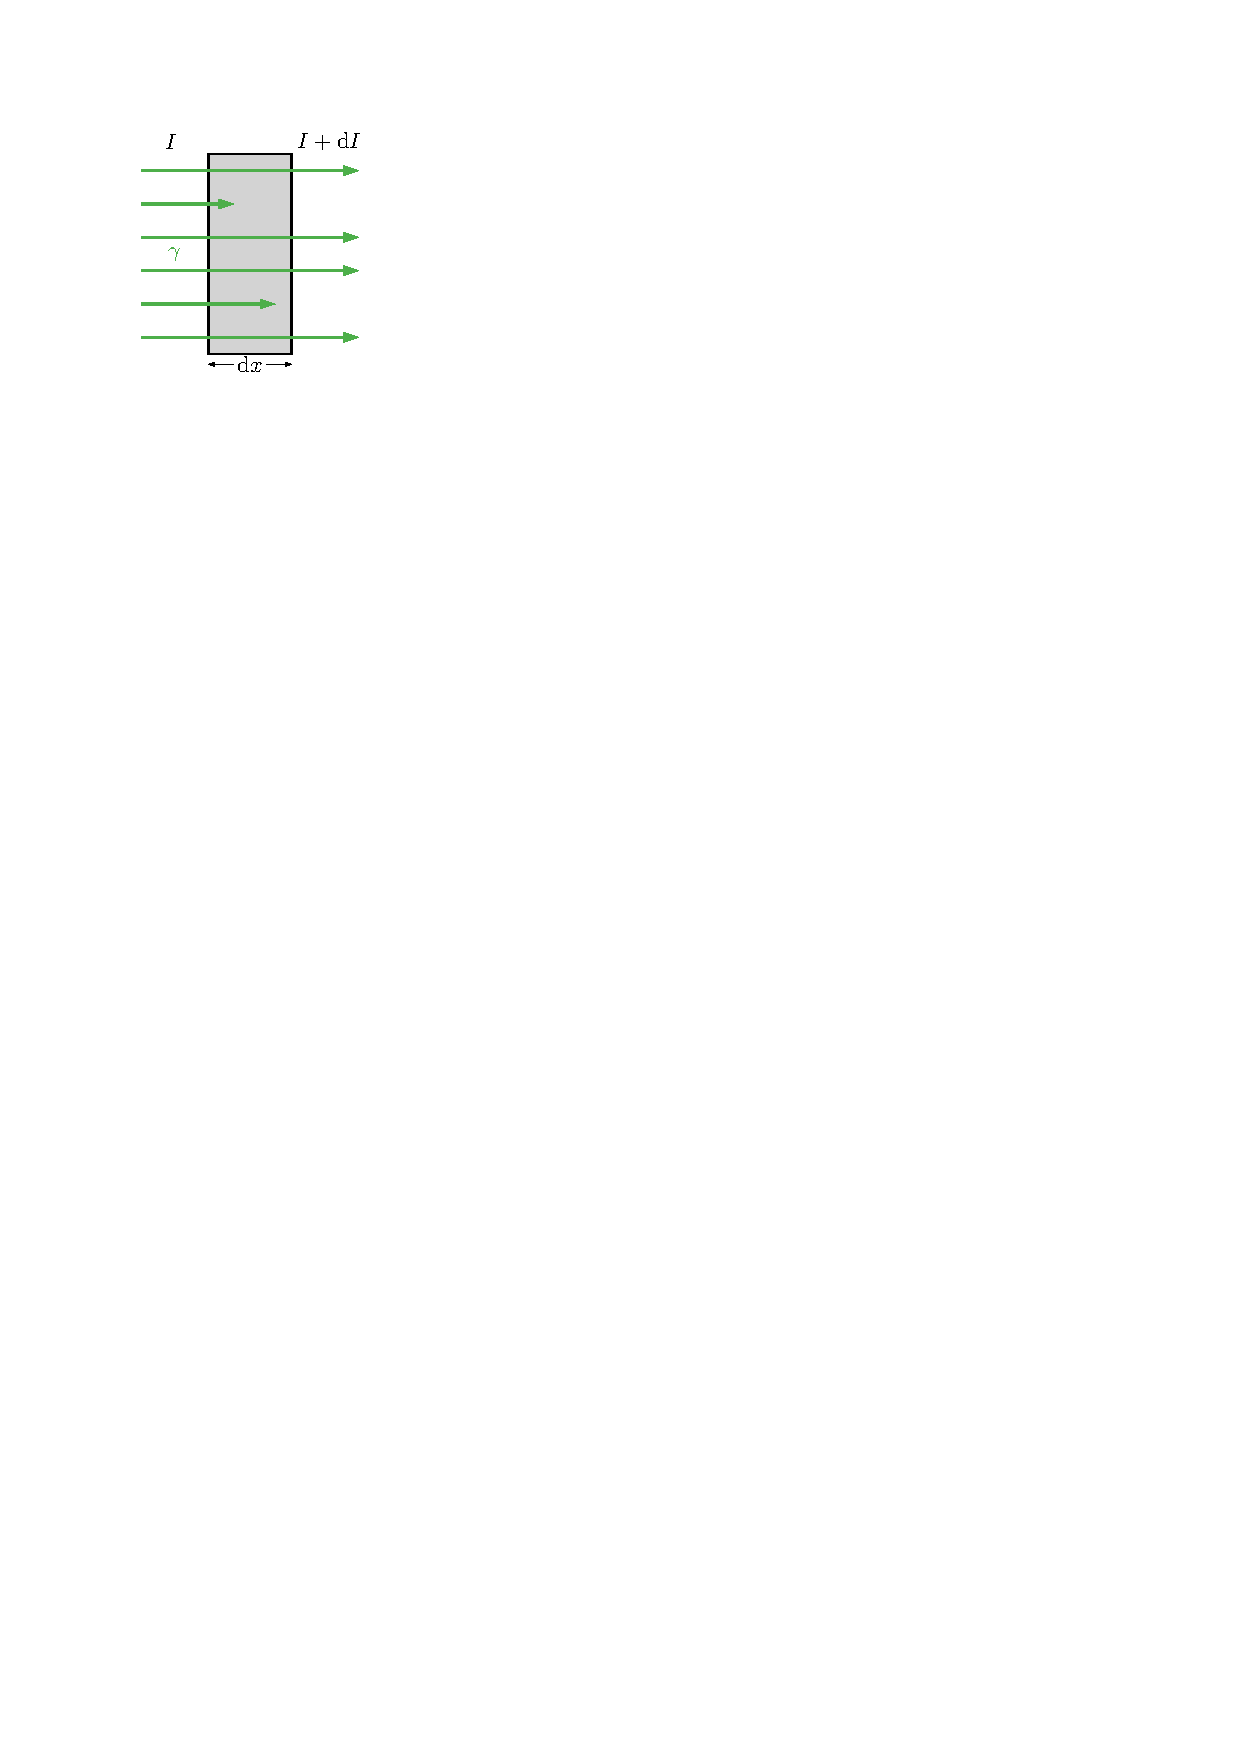
\includegraphics{./figures/lambert_beer.pdf}
			\end{center}
			\begin{align*}
				\mathrm{d} I = - \mu I \mathrm{d}x
			\end{align*}
			
			Lambert-Beer law:
			\begin{align*}
				I(x) = I_0 \, e^{-\mu x}
			\end{align*}
	\end{columns}
\end{frame}

\begin{frame}{Absorption coefficient}
	\begin{itemize}
		\item absorption coefficient
		\begin{align*}
			\mu = n \sigma
		\end{align*}
		density of atoms $n$, total absorption/scattering cross section $\sigma$ per atom
		
		\item mean free path
		\begin{align*}
			\lambda = \frac{1}{\mu}
		\end{align*}
		
		\item cross section per atom ($Z$?) (processes independent)
		\begin{align*}
			\sigma = \sigma_\mathrm{photo} + Z \cdot \sigma_\mathrm{Compton} + \sigma_\mathrm{pair}
		\end{align*}
		
		\item contains dependence on material/photon energy
	\end{itemize}	
\end{frame}

\section{Interaction processes}

\begin{frame}{Interaction processes}
	PDG cross section plot?\\
	dominant interactions at photon energies $E_\gamma$?\\
	dominant interactions for atomic number $Z$?
	\begin{itemize}
		\item photoelectric effect: $E_\gamma < \SI{1}{MeV}$
		\item Compton scattering: $E_\gamma \approx \SI{1}{MeV}$
		\item pair production: $E_\gamma > \SI{1}{MeV}$
	\end{itemize}
\end{frame}

\subsection{Photoelectric effect}

\begin{frame}{Photoelectric effect}
	\begin{itemize}
		\item absorption of photon by atomic electron (illustration) (free electron -- forbidden: recoil momentum)
		\item $E = h \nu - E_\mathrm{b}$
		\item complete transfer of energy
		\item cross section -- shell structure
		\begin{itemize}
			\item absorption-edges
			\item K-shell dominant for high energies
		\end{itemize}
		nonrelativistic but $E_\gamma > E_\mathrm{b, K}$:
		\begin{align*}
			\sigma_\mathrm{photo} = \frac{32 \pi}{3} \sqrt{2} r_\mathrm{e}^2  \alpha^4  Z^5 \left( \frac{m_\mathrm{e} c^2}{E_\gamma}\right)^\frac{7}{2} 
		\end{align*}		
	\end{itemize}
\end{frame}

\begin{frame}{Sketch}

\end{frame}


\subsection{Compton scattering}

\begin{frame}{Compton scattering}
	\begin{itemize}
		\item
	\end{itemize}
\end{frame}

\subsection{Pair production}

\begin{frame}{Pair production}
	\begin{itemize}
		\item
	\end{itemize}
\end{frame}



\section{Electromagnetic showers}

\section{Detector concepts}

\begin{frame}{Detector concepts}
	\begin{itemize}
		\item PMT
	\end{itemize}
\end{frame}


\begin{frame}{Bibliography}
	\begin{thebibliography}{1000}
		\bibitem[Leo]{leo}
			W.\ R.\ Leo,
			\emph{Techniques for Nuclear and Particle Physics Experiments},
			Springer (1994).
		
		\bibitem[Sieg]{siegbahn}
			C.\ M.\ Davisson,
			\emph{Interaction of $\gamma$-Radiation with Matter},
			published in K.\ Siegbahn (ed.),
			\emph{Alpha- Beta- and Gamma-Ray Spectroscopy}, North-Holland Publishing Company (1979).
		
		\bibitem[PDG]{pdg}
	\end{thebibliography}
\end{frame}

\beginbackup

\begin{frame}{Appendix}
\end{frame}

\backupend

\end{document}